\documentclass[11pt]{article}

%\usepackage[english]{babel}
\usepackage[utf8]{english}

%\usepackage[english,vietnam]{babel}
%\usepackage[utf8x]{inputenc}

%\usepackage[utf8]{inputenc}
%\usepackage[francais]{babel}
\usepackage{a4wide,amssymb,epsfig,latexsym,multicol,array,hhline,fancyhdr}
\usepackage{lastpage}

\usepackage[lined,boxed,commentsnumbered]{algorithm2e}
\usepackage{enumerate}
\usepackage{color}
\usepackage{graphicx}							% Standard graphics package
\usepackage{array}
\usepackage{tabularx}
\usepackage{multirow}
\usepackage{multicol}
\usepackage{rotating}
\usepackage{graphics}
\usepackage[a4paper,left=2cm,right=2cm,top=1.8cm,bottom=2.8cm]{geometry}
\usepackage{setspace}
\usepackage{epsfig}
\usepackage{tikz}
\usetikzlibrary{arrows,snakes,backgrounds}
\usepackage{hyperref}
\hypersetup{urlcolor=blue,linkcolor=black,citecolor=black,colorlinks=true} 
%\usepackage{pstcol} 								% PSTricks with the standard color package



%\usepackage{amsmath,amsfonts,amssymb,amsthm,epsfig,epstopdf,titling,url,array}
\usepackage{tabularx,ragged2e}
\usepackage{booktabs}
\usepackage{graphicx}
\usepackage{float}

%for long algorithm
\usepackage{algorithmicx}
%\addtolength\textheight{-32\baselineskip}
%\addtolength\paperheight{-32\baselineskip}
%\pdfpageheight\paperheight
%\renewcommand\labelenumi{\textbf{\theenumi) }}
%\usepackage[linesnumbered,algoruled,lined,boxed]{algorithm2e}
%\usepackage{algorithm}% http://ctan.org/pkg/algorithms
\usepackage{algpseudocode}% http://ctan.org/pkg/algorithmicx
\usepackage{varwidth}% http://ctan.org/pkg/varwidth

\algnewcommand\algorithmicinput{\textbf{Input:}}
\algnewcommand\INPUT{\item[\algorithmicinput]}
\algnewcommand\algorithmicoutput{\textbf{Output:}}
\algnewcommand\OUTPUT{\item[\algorithmicoutput]}


\algtext*{EndIf}% Remove "end if" text
\algtext*{EndFor}% Remove "end if" text
\algtext*{EndWhile}% Remove "end if" text

\newtheorem{theorem}{{\bf Định lý}}
\newtheorem{property}{{\bf Tính chất}}
\newtheorem{proposition}{{\bf Mệnh đề}}
\newtheorem{corollary}[proposition]{{\bf Hệ quả}}
\newtheorem{lemma}[proposition]{{\bf Bổ đề}}
\newtheorem{observation}[proposition]{{\bf Nhận xét}}

%%ensembles de nombres
\def\NP{$\mathcal{NP}$}
\def\N{\mathbb{N}}
\def\Z{\mathbb{Z}}
\def\R{\mathbb{R}}
\def\Q{\mathbb{Q}}


%\usepackage{fancyhdr}
\setlength{\headheight}{40pt}
\pagestyle{fancy}
\fancyhead{} % clear all header fields
\fancyhead[L]{
 \begin{tabular}{cc}
    \begin{picture}(25,15)(0,0)
    \put(0,-8){
\includegraphics[width=8mm, height=8mm]{hcmut.png}}
   \end{picture}
	\begin{tabular}{l}
		\textbf{\bf \ttfamily Ho Chi Minh University of Technology}\\
		\textbf{\bf \ttfamily Faculty of Computer Science and Engineering}
	\end{tabular} 	
 \end{tabular}
}
\fancyhead[R]{
	\begin{tabular}{l}
		\tiny \bf \\
		\tiny \bf 
	\end{tabular}  }
\fancyfoot{} % clear all footer fields

\fancyfoot[R]{\scriptsize \ttfamily Page {\thepage}/\pageref{LastPage}}
\renewcommand{\headrulewidth}{0.3pt}
\renewcommand{\footrulewidth}{0.3pt}


\begin{document}

\begin{titlepage}
\begin{center}
\noindent Ho Chi Minh University of Technology\\
Faculty of Computer Science \& Engineering\
\end{center}

\vspace{1cm}

\begin{figure}[h!]
\begin{center}

\includegraphics[width=3cm]{hcmut.png}
\end{center}
\end{figure}

\vspace{1cm}


\begin{center}
\begin{tabular}{c}
\multicolumn{1}{l}{\textbf{{\Large SOFTWARE ENGINEERING}}}\\
~~\\
\hline
\\
\multicolumn{1}{l}{\textbf{{\Large ASSIGNMENT}}}\\
\\
\textbf{{\Huge RESTAURANT POS 2.0}}\\
\\
\hline
\end{tabular}
\end{center}

\vspace{3cm}

\begin{minipage}[t]{0.60\linewidth}
Lecturer \\ 
Dr. Quan Thanh Tho, Associate Professor
\end{minipage}
\begin{minipage}[t]{0.40\linewidth}
Students\\
Nguyen Bao Phuc - 1712674\\
Pham Ngoc Manh - 1813045\\
Lam Minh Vinh - 2120082\\
Pham Ngoc Hau - 1911136\\
Nguyen Huu Thuan - 1920060\\
\end{minipage}

\end{titlepage}

\newpage

\tableofcontents 
\cleardoublepage
\pagenumbering{arabic}          % to start the page numbering
\pagebreak
%-------------
\section{Report 1}
    \subsection{Introduction}
    \subsubsection*{Project context}
    During the COVID-19 crisis, people are paying more attention to their health and convenience, meanwhile, software engineering shows its myriad advantages by assisting and promising people unique ways of experiencing the outside environments. Concerning the restaurant business, an application can automate tedious and insecure tasks such as giving customer the menu, offline payment, reserving a table by phone,... can make both the restaurant staffs and customers easier and safer. This project aims to deliver to the restaurant's owner a useful application, which has the ability of automating the ordering and processing meals procedure without directly communicating between customers and restaurant staffs to reduce wasted effort and protect people from the coronavirus pandemic.
    \subsubsection*{Project stakeholders}
    \begin{itemize}
        \item \textbf{Customer:} Can be considered as the major user class of this system. In Restaurant POS 2.0, customers can select their desired meals via a friendly menu, order foods, pay for their invoice, and give back some feedback or surveys. 
        \item \textbf{Clerk:} Provide their services to customers by confirming orders, processing customers' feedback, and serving meals to customers after being notified by the kitchen staff via the application.
        \item \textbf{Point-of-sale terminals:} Including third-party payment service, staffs that have a responsibility of processing customers' order before sending a request to the kitchen staffs.
        \item \textbf{Chef:} Receiving requests from others staff, making food, and calling clerk to serve the ordered meal to the customer.
        \item \textbf{Manager}: Manage system's operation as well as customer's feedbacks.
    \end{itemize}
    \subsubsection*{Project objectives}
    In this project, we try to obtain results corresponding to the objectives are as follows:
    \begin{itemize}
        \item Customer can check the menu and request for the item that they want.
        \item Customer can access the application via a QR code.
        \item Clerk can receive customers' request without meeting and asking customer directly.
        \item Restaurant staff can check and confirm customer orders.
        \item Kitchen staff can receive the customer's order after restaurant staff confirms it.
        \item Recommendation system suggests user to choose some trending or discounted meals.
    \end{itemize}
    \subsubsection*{Project scope}
    In terms of project scope, there are three main points:
    \begin{itemize}
        \item Implement a responsive web application for both computer and mobile phone.
        \item Design a database to persist user or food information.
        \item Implement a recommendation system that can suggest user to choose meal from a menu, which can highly increase user experiences. Some basic machine learning techniques will be used.

    \end{itemize}
    \subsubsection*{Technologies}
    \begin{itemize}
        \item Platform: Responsive web application.
        \item Back-end: NestJS framework.
        \item Front-end: ReactJS framework.
        \item Database: MongoDB.
    \end{itemize}
    \subsection{Functional Requirement}
        \subsubsection*{Functional Requirement}
        \begin{itemize}
            \item Payment: The customer can choose the payment method to pay for their order.
            \item Table reservation: Clerk can check the status of the reservation, customers can choose table.
            \item Food Ordering: Customers can view food and select food that they want, clerks check the status of the ordering, and the chef receives orders to prepare food.
            \item Billing: Make bill for customer's order.
            \item Checkout: Check customer's order and know your money will pay, include scan item, calculate total.
            \item Alerts: Alert warning if the customer choose a reserved table, a payment error occurs,...
            \item Scan QR Code: The system generates a QR code, Customer can scan that QR code to log-in to the system.
            \item Customer Management: Customers send feedbacks about restaurant’s service. Manager can view feedbacks and sale report for each day, week, month.
        \end{itemize}
        \subsection{Non-Functional Requirement}
        \subsubsection*{Security}
        \begin{itemize}
            \item Users can access the application without creating a username and password. For takeaway orders, users have to provide at least their name, phone number, email,.... 
            \item Restaurant staffs must have their unique username/password pair. And only can access the application by the correct username and password.
        \end{itemize}
        \subsubsection*{Maintainability}
        \begin{itemize}
            \item The system operates 24/7, maintenance is 1 time / month.
            \item Each maintenance time is not more than 4 hours.
            \item Maintenance preservation must be notified at least 3 days.
        \end{itemize}
        \subsubsection*{Reliability}
        \begin{itemize}
            \item Correctly connect customers with their orders.
            \item Calculate the correct amount the customer needs to pay.
        \end{itemize}
        \subsubsection*{Concurrency and capacity}
        \begin{itemize}
            \item The current transactions is about 300 orders per day.
            \item Page transition time under 3 seconds.
        \end{itemize}
        \subsubsection*{User interface}
        \begin{itemize}
            \item The system should be usable from a mobile device, a tablet device or a normal computer/ laptop.
            \item Maximum 5 steps to complete a function.
            \item Up to 1 hour to use the system fluently.
        \end{itemize}
        \subsubsection*{Scalability}
        \begin{itemize}
            \item The system should be extendable to use in multiple restaurants in the future.
        \end{itemize}
        % \begin{itemize}
        %     \item The system should allow non-direct contact between Clerks and Customers.
        %     \item The system should be implemented using Web technology and QR code, so customers will not have to install apps.
        %     \item The system should be usable from a mobile device, a tablet device or a normal computer/laptop.
        %     \item The system should be extendable to use in multiple restaurants in the future.
        %     \item The current transactions are about 300 orders per day.
        % \end{itemize}
        \subsubsection*{Use-case diagram}
        \begin{figure}[h]
            \centering
            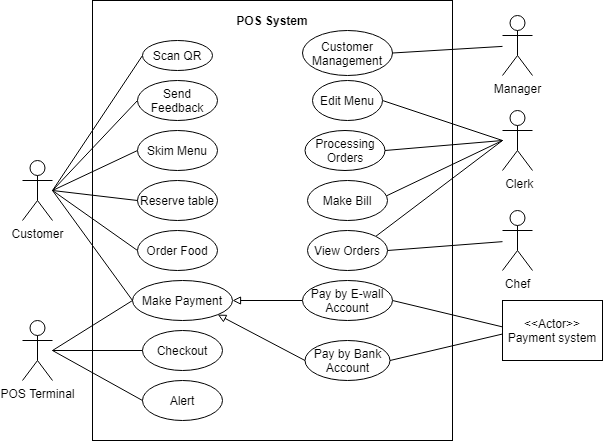
\includegraphics[scale=0.8]{Use-case diagram/Use-case-diagram.png}
            \setlength{\parskip}{8pt}
        \end{figure}
\pagebreak
%----------------

    \subsection{Use-case description}
    %\setlength{\parskip}{2pt}
    %\begin{minipage}{\dimexpr\textwidth-2cm}
    %\setlength{\parskip}{2pt}
    %\end{minipage}
        \begin{enumerate}
            \item[a.] Table reservation 
        \end{enumerate}
    \begin{figure}[h]
        \centering
        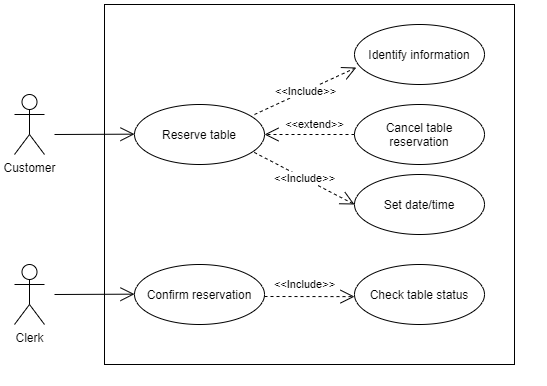
\includegraphics[scale=0.8]{Use-case diagram/TableReservation.png}
        \setlength{\parskip}{8pt}
    \end{figure}
        
    \begin{table}[!h]
    \centering
        \begin{tabular}{|c|p{14cm}|}
        \hline
        \textbf{Name}  & \textbf{Table reservation} \\
        \hline
        \textbf{Actor} & Clerks and customers\\
        \hline
        \textbf{Description} & Clerk can check the status of the reserved table and confirm the identity of the customer.\\
        {} & {Customers can message, send notifications, and choose any seats via home page, they can also cancel the reservation}.\\
        \hline
        \textbf{Preconditions} & Customers need to access to home page.\\
        {} & Clerks need to have an account and log in first.\\
        \hline
        \textbf{Normal flow} & 1. Customers go to home page of website by URL and clerks log in the website application.\\
        {} & 2. In the section of table reservation, the website presents a page with many results in available seats.\\
        {} & 3. Customers can choose  the remaining seats they want\\
        {} & 4. Customers have to identify their information (phones, names, ID, date-time).\\
        {} & 5. Clerks can check the information of customers and the table they reserved, and confirm the result.\\
        \hline
        \textbf{Exceptions} & Exception 1: At step 5: Customer can cancel the table they reserved.\\
        {} & Exception 2: At step 4: if customers have not identified all these information, the reservation cannot be executed.\\
        {} & Exception 3: At step 3: If customers have chosen the reserved table, they cannot input the step 4.\\
        {} & Exception 4 :At step 1, if Clerks have not logged into their account , they cannot operate the system.\\
        \hline
        \textbf{Alternative flow} & Alternative 1, Exception 2 : Website can notify the customers they have not identified their information yet.\\
        {}  & Alternative 2, Exception 3 : Website can notify the status of the table.\\
        \hline
        \end{tabular}
    \end{table}
\pagebreak
%---------------
    
    \begin{enumerate}
        \item[b.] Food Ordering 
    \end{enumerate}
    \begin{figure}[h]
        \centering
        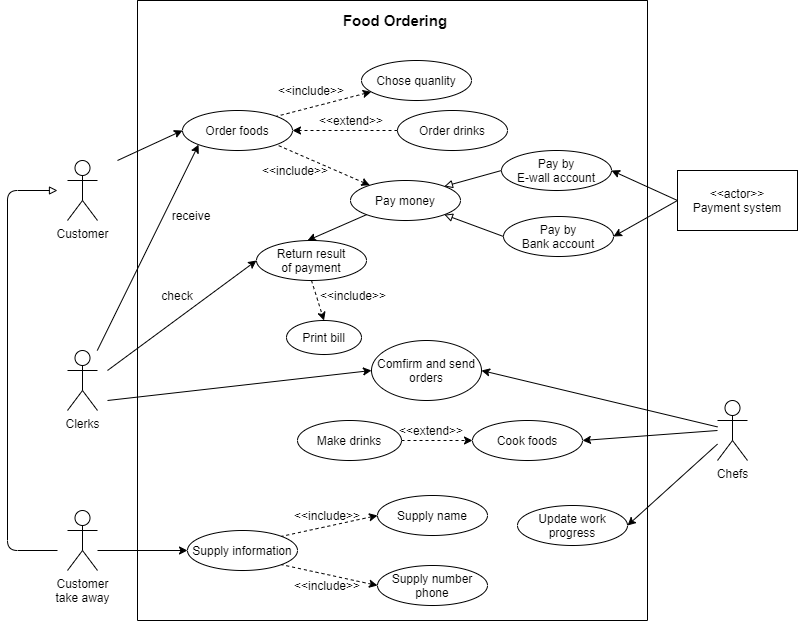
\includegraphics[scale=0.6]{Use-case diagram/FoodOrdering.png}
    \end{figure}
    \begin{table}[!h]
    \centering
        \begin{tabular}{|c|p{14cm}|}
        \hline
        \textbf{Name}  & \textbf{Food ordering} \\
        \hline
        \textbf{Actor} & Clerks, customers, chefs and payment system\\
        \hline
        \textbf{Description} & Clerks receive orders, check payment, confirm orders and send orders to chefs.\\
        {} & Customers chose food or drink, pay money, and get food.\\
        {} & Chefs receive orders and cook food or make drinks.\\
        {} & Payment system make transaction and return result to clerks.\\
        \hline
        \textbf{Preconditions} & Clerks have an account and login to home page.\\
        {} & Customers access to home page.\\
        {} & Chefs are ready.\\
        {} & Payment system is available.\\
        \hline
        \textbf{Normal flow} & 1. Customers click on Menu button to go to Menu page.\\
        {} & 2. System gets and displays list of food.\\
        {} & 3. Customers chose foods or drinks and quantity via Menu page.\\
        {} & 4. Customers chose pay money via payment system by E-wall account or by Bank account. Payment system will make transaction and return result to clerks.\\
        {} & 5. Clerks receive orders from customers, check result of payment system, confirm order.\\
        {} & 6. System print bill and send orders to chefs.\\
        {} & 7. Chefs receive orders, start cook foods or make drinks and update work progress.\\
        {} & 8. Clerk mark the order as completed.\\
        \hline
        \textbf{Exceptions} & Exception 1: At step 3: If result of payment system is failed, customers will refuse orders.\\
        \hline
        \textbf{Alternative flow} & Alternative 1, Exception 1: Payment system notice failed transaction to customers and give reasons.\\
        \hline
        \end{tabular}
    \end{table}
\cleardoublepage
%-----------
    \begin{enumerate}
        \item[c.] Customer management
    \end{enumerate}
    \begin{figure}[h]
        \centering
        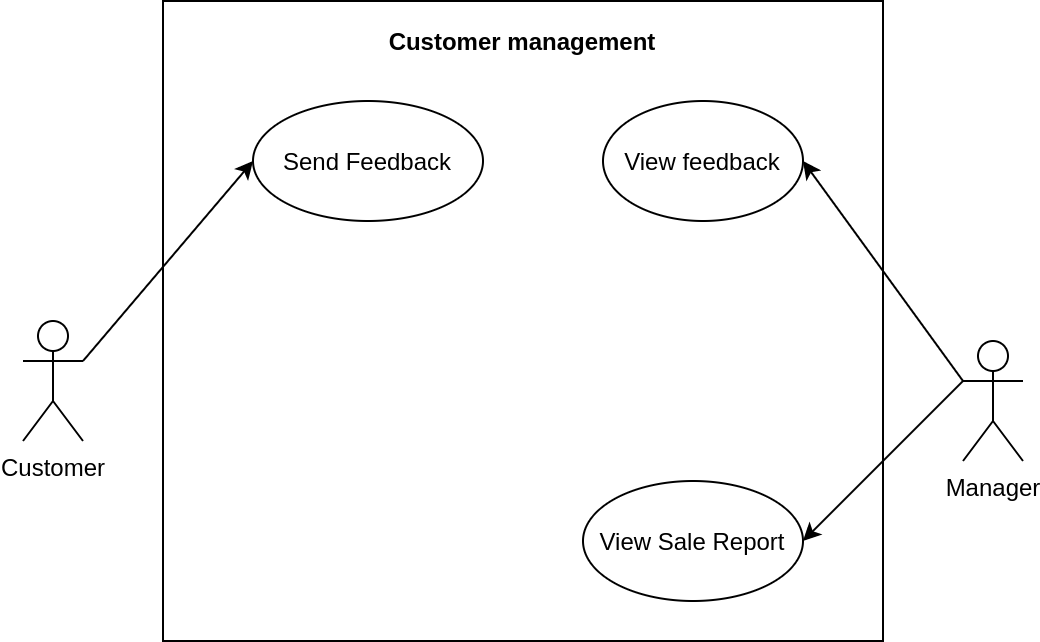
\includegraphics[scale=0.3]{Use-case diagram/CustomerManagement.png}
    \end{figure}
    \begin{table}[!h]
    \centering
        \begin{tabular}{|c|p{14cm}|}
        \hline
        \textbf{Name}  & \textbf{Food ordering} \\
        \hline
        \textbf{Actor} & Manager, customer\\
        \hline
        \textbf{Description} & Customers send feedbacks about restaurant's service.\\
        {} & Manager can view feedbacks.\\
        {} & Manage can view sale report for each day, week, month.\\
        \hline
        \textbf{Preconditions} & Managers have an admin account and login to home page.\\
        {} & Customers access to the Feedback page.\\
        \hline
        \textbf{Normal flow} & 1. Customers type their feedbacks in a feedback section.\\
        {} & 2. System stores and sends feedback notification to manager. \\
        {} & 3. Manager inspect customer's feedbacks in a customer feedback section.\\
        {} & 4. Manager can view the sale report by clicking on the Sale report button. \\
        {} & 5. System will calculate and send to report to manager as a pdf file. \\ 
        \hline
        \textbf{Exceptions} & Exception 1: At step 4: If the system does not have any sale record, manager can not view sale report.\\
        \hline
        \textbf{Alternative flow} & Alternative 1, Exception 1: The system can notify the sale status to the manager.\\
        \hline
        \end{tabular}
    \end{table}
%%%%%%%%%%%%%%
\cleardoublepage
\section{Report 2}
    \subsection{Activity diagram}
        \begin{enumerate}
            \item[a. ] Table Reservation
        \end{enumerate}
            \begin{figure}[!h]
                \centering
                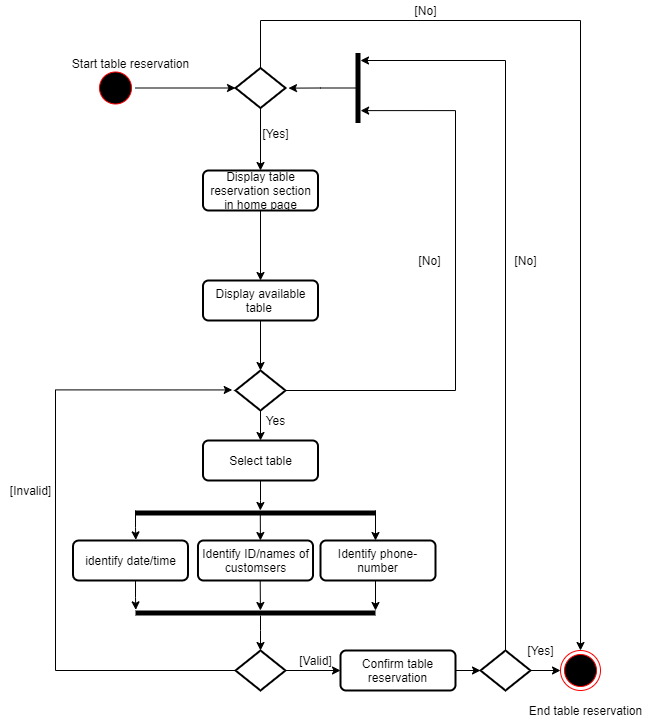
\includegraphics[scale=0.58]{Activity diagram/TableReservation.png}
            \end{figure}
            \textit{Description:}
            \begin{itemize}
                \item In the first stage, there is a decision node that whether customers are able to access to table reservation or not, which means it can create the flow of output when they think reservation is not necessary.
                \item When customers access to table reservation section,the application show the available seats.
                \item Subsequently, a decision node 2 appears, if none of table is unavailable or  customers unsatisfied with the remaining available seats, they can return to decision node 1.In contrast, they can select the table.
                \item After selecting the table, customers have to declare their information such as date/time, names, and phone-number.
                \item After that,decision note 3 will show that if one of these information is invalid or unidentified, the application will return the decision note 2 and system will show the notification about that.In contrast, they obviously
                confirm table reservation in the next step.
                \item After confirmation step, the existence of decision note 4 means that if customers accept the confirmation.If not,they will return decision note 1.
            \end{itemize}
            
        \begin{enumerate}
            \item[b. ] Food Ordering
        \end{enumerate}
            \begin{figure}[!h]
                \centering
                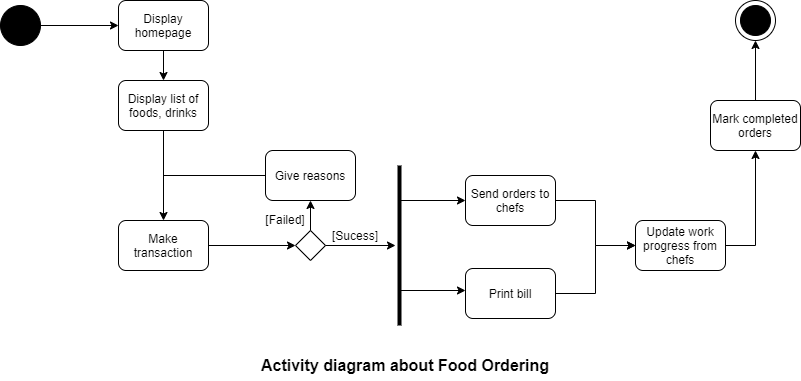
\includegraphics[scale=0.58]{Activity diagram/FoodOrdering.png}
            \end{figure}
            \textit{Description:} System will display homepage. After customer click on menu button, system will display list of foods and drinks to customer order. Then, customer choose pay money, system make a  transaction. If transaction is fail, system will give reason for customer. Otherwise, system will print bill, send order to chefs. Update progress of order and mark completed when chefs done.
        \begin{enumerate}
            \item[c. ] Skin Menu
        \end{enumerate}
            \begin{figure}[!h]
                \centering
                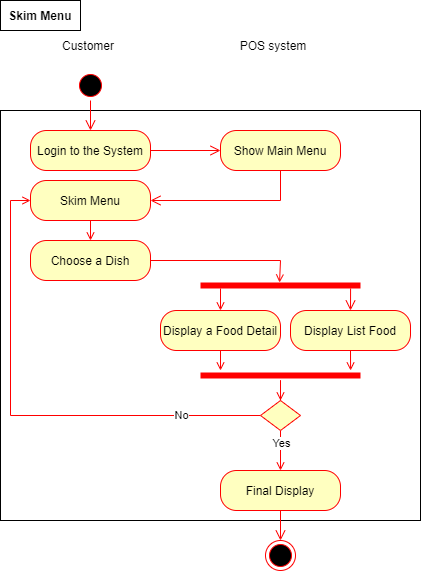
\includegraphics[scale=0.53]{Activity diagram/Skim Menu.png}
            \end{figure}
        \cleardoublepage
            \textit{Description:} 
            \begin{itemize}
                \item The customer logs into the system.
                \item The system displays the main menu.
                \item Customer can skim the menu and choose their favorite dishes.
                \item The system displays the customer's dishes according to the list of related dishes or the details of a single dish.
                \item If customer can't find the dish, they can skim the menu and choose another dish again.
            \end{itemize}
        \begin{enumerate}
            \item[d. ] Payment
        \end{enumerate}
            \begin{figure}[!h]
                \centering
                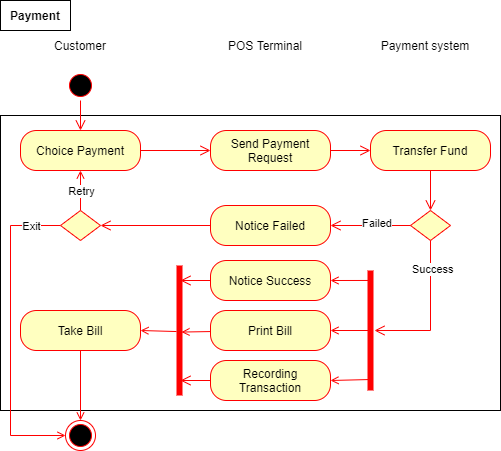
\includegraphics[scale=0.6]{Activity diagram/Payment.png}
            \end{figure}
            \textit{Description:}
            \begin{itemize}
                \item Display the payment page.
                \item Customer choose payment gateway and transfer money.
                \item The system updates the payment process.
                \item Show paid if payment is successful, save the transaction and issue an electronic invoice to the customer.
                \item Show failed payment and ask customer to try again or exit.
            \end{itemize}
            \cleardoublepage
        \begin{enumerate}
            \item[e. ] Checkout
        \end{enumerate}
            \begin{figure}[!h]
                \centering
                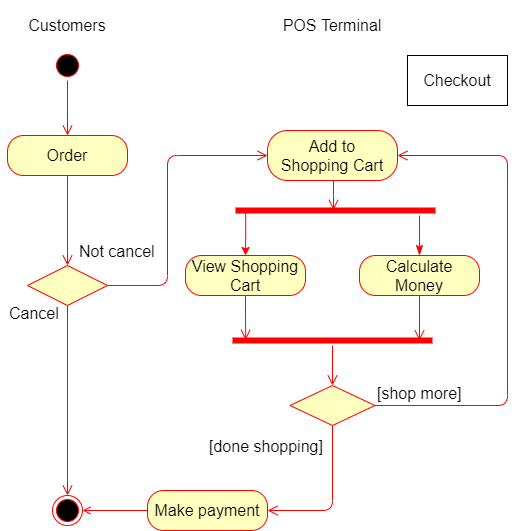
\includegraphics[scale=0.45]{Activity diagram/Checkout.png}
            \end{figure}
            \textit{Description: }When the customer orders something(food, table), the pos terminal will display the shopping cart and calculate the total amount. If the customer wants to choose more, the POS terminal will display the menu, and vice versa if the customer completes the purchase and presses pay, the pos terminal will display the payment system.
        \begin{enumerate}
            \item[f. ] Alert
        \end{enumerate}    
            \begin{figure}[!h]
                \centering
                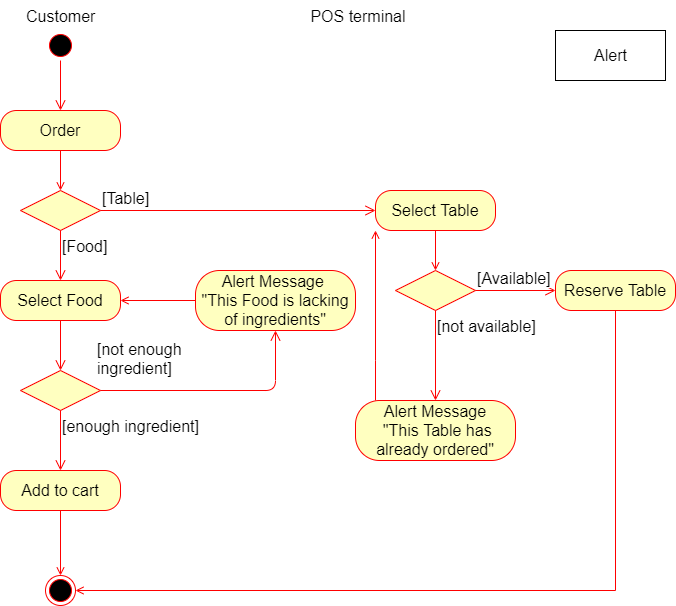
\includegraphics[scale=0.45]{Activity diagram/Alert.png}
            \end{figure}
            \textit{Description: }When customer orders, if the ingredient of the food is not enough, or the table is not available. The POS system will alert about this error and require customer choose again.
    \cleardoublepage
    \subsection{Sequence diagram}
        \begin{enumerate}
            \item[a.] Table reservation
        \end{enumerate}
            \begin{figure}[!h]
                \centering
                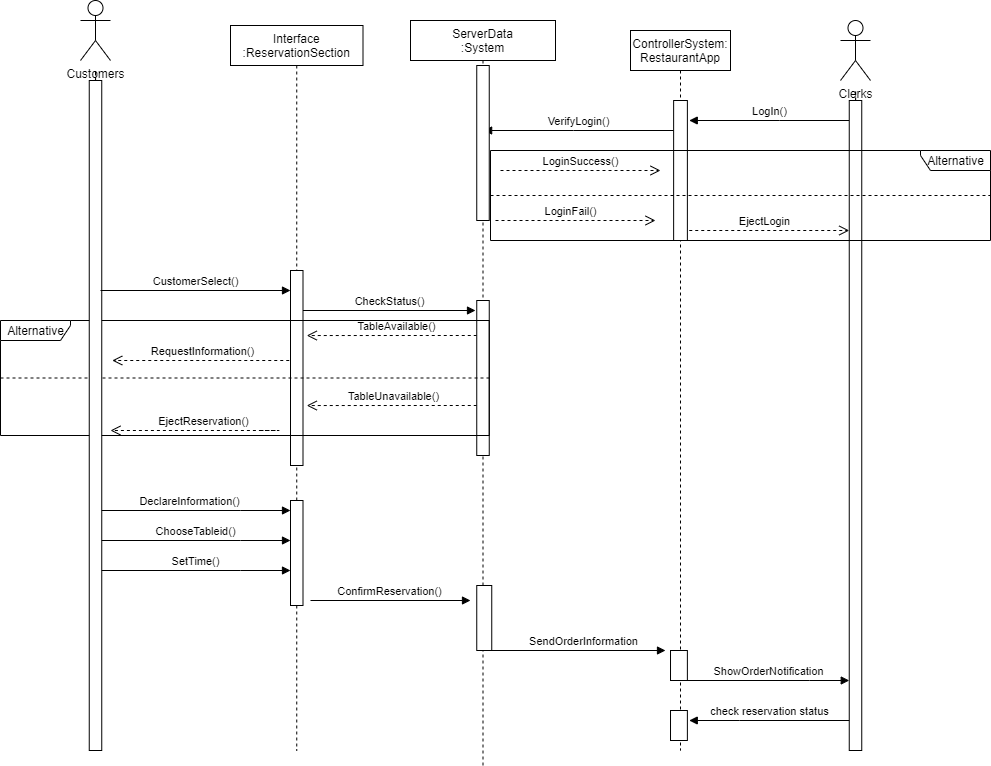
\includegraphics[width=16cm]{Sequence diagram/TableReservation.png}
            \end{figure}
        \cleardoublepage
        \begin{enumerate}
            \item[b.] Food Ordering
        \end{enumerate}
            \begin{figure}[!h]
                \centering
                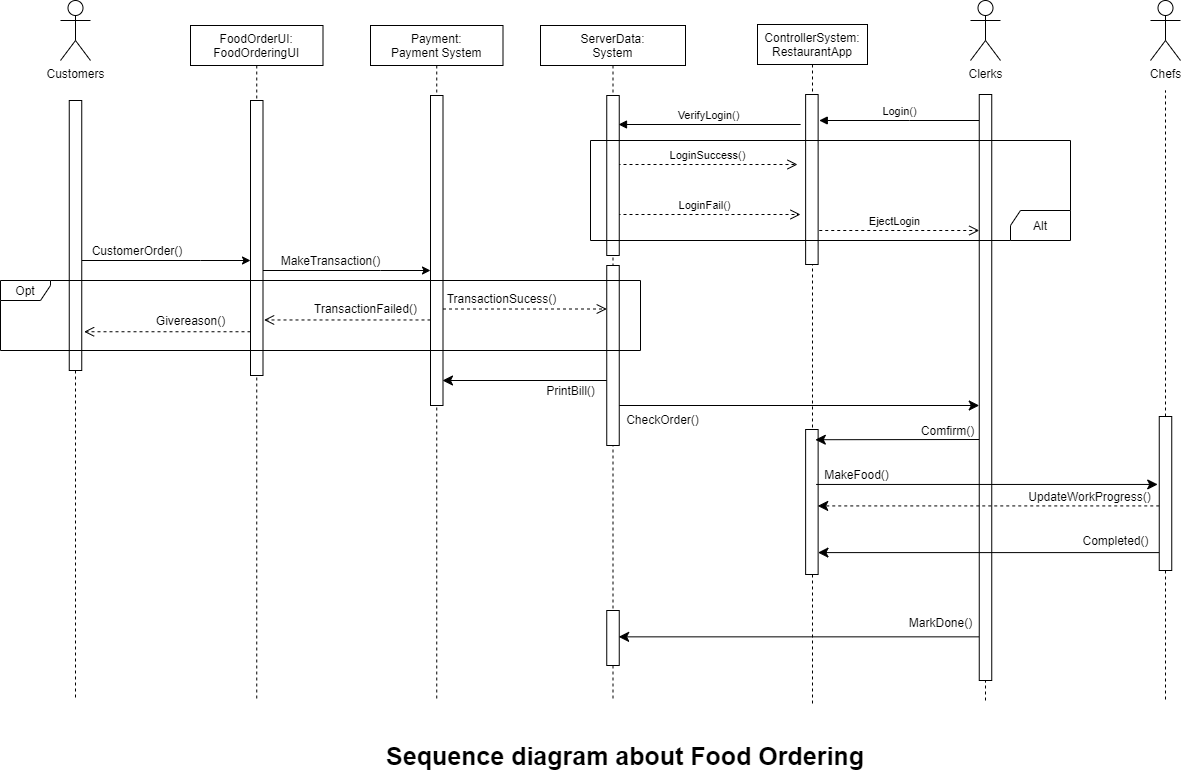
\includegraphics[width=16cm]{Sequence diagram/FoodOrdering.png}
            \end{figure}
    \cleardoublepage
    \subsection{Class diagram}
    \begin{figure}[!h]
        \centering
        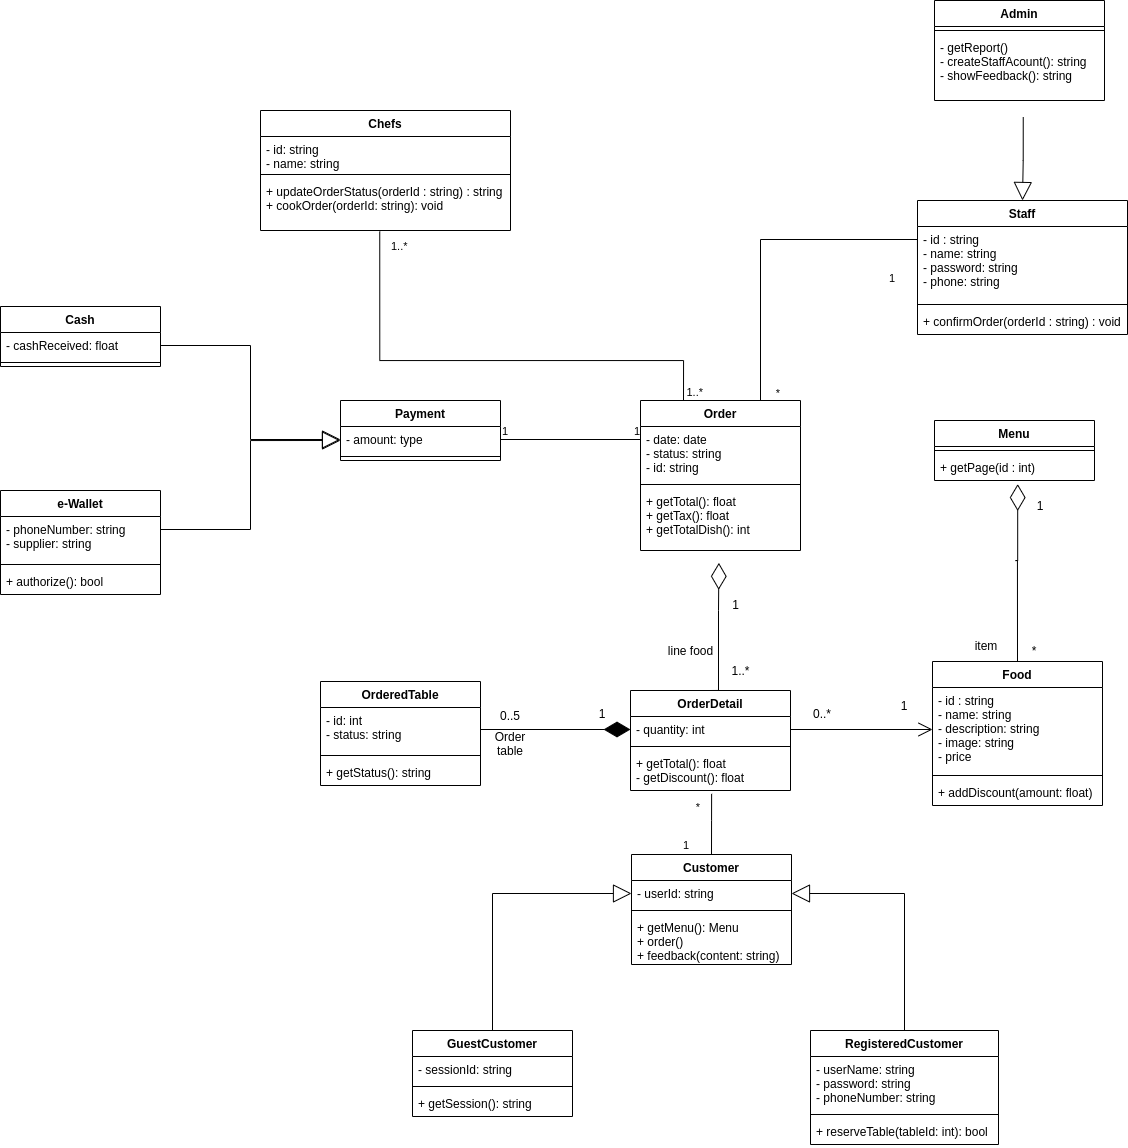
\includegraphics[width=17cm]{ClassDiagram.png}
    \end{figure}
%%%%%%%%%%%%%%%%
\cleardoublepage
\section{Report 3}
    \subsection{Describe architectural approach (MVC)}
    \begin{figure}[!h]
        \centering
        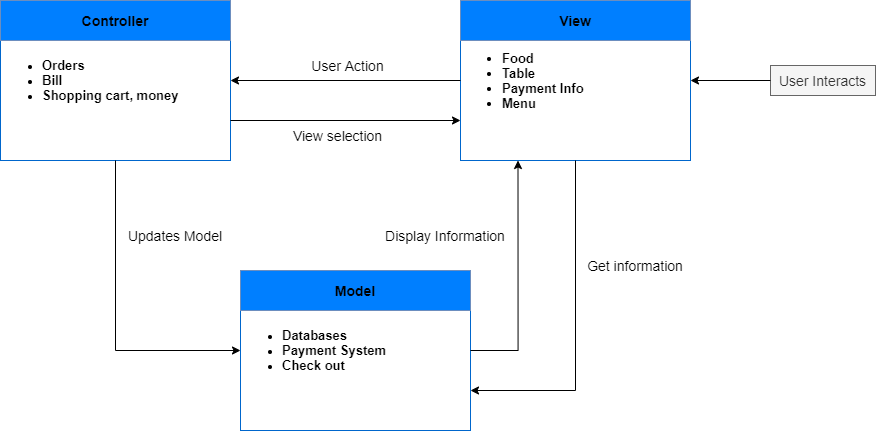
\includegraphics[scale=0.52]{MCV.png}
    \end{figure}
    \textit{Description:}
    \begin{itemize}
        \item The system will display the homepage. When a user interacts with the system, the action of user will send required to retrieve the data from the model and send the request to the controller if any new action is updating from the data. The controller collects the action from View and sends information updated to Model for process and manipulation, then sends the update to View.
        \item Controller: NestJS framework (Back-end). View: ReactJS framework (Front-end). Modal: MongoDB (Database).
        \item For example, Customer skims menu to choose the food, View send a request to the Model (database) to display food information, then the customer chooses the food, the action will send the Controller, the Controller will update the information to the Model (check out: add shopping cart, money) and the Model sends update information to the View.
    \end{itemize}
    \newpage
    \subsection{Implementation diagram (Component Diagram)}
    \begin{figure}[!h]
        \centering
        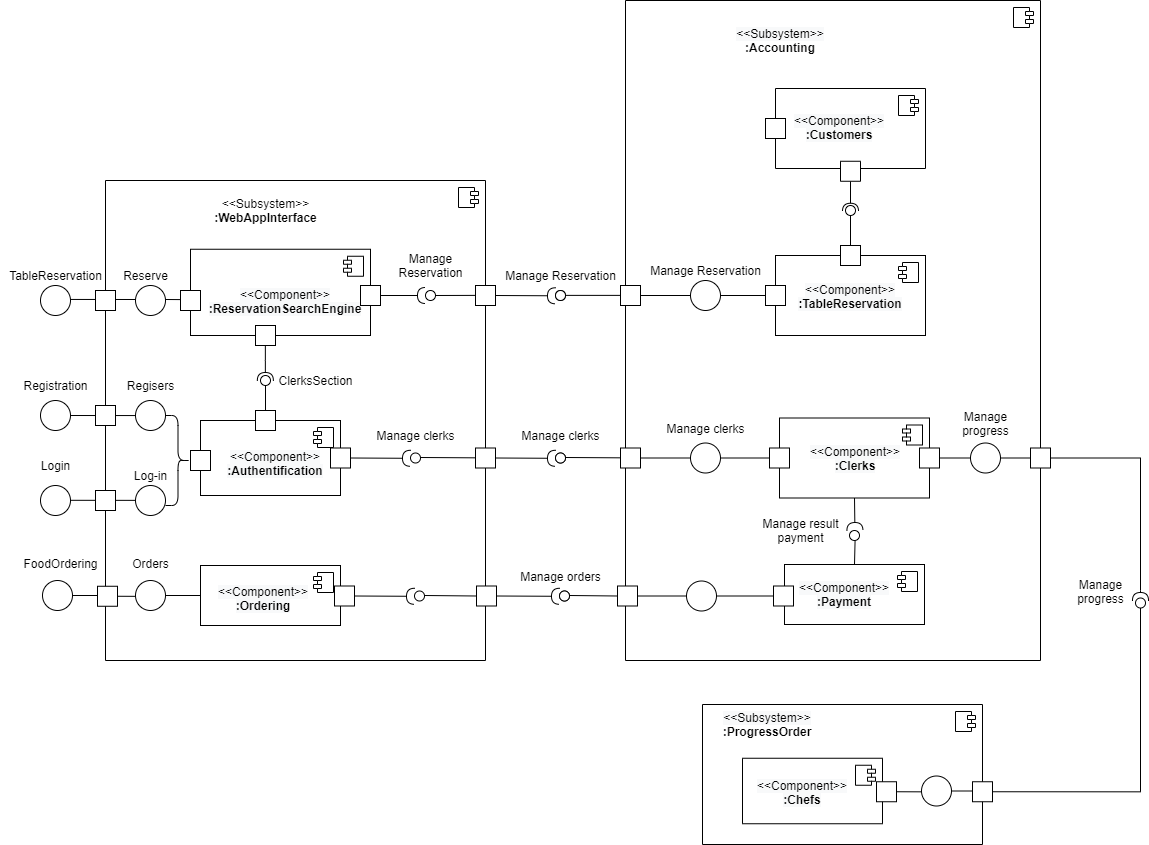
\includegraphics[width=17cm]{ComponentDiagram.png}
    \end{figure}
    \textit{Description:}
    \begin{itemize}
        \item WebAppInterface subsystem contains components related to ReservationSearchEngine, Authentication, and Ordering. Search Engine component allows to search or browse items by table reservation such as status (reserved or unreserved), Identity (table numbering). Authentication component allows clerks to create account, login, or logout and binds customer to some account. Ordering component allows customer order foods, drinks, and manage that orders.
        \item Accounting subsystem provides three interfaces - Manage Reservation, Manage Clerks, and Manage Orders. TableRevervation component allows Customer check and manage table reservation. Clerks component is used in oder to manage clerks on restaurant. Finally, Payment component manage ordering of Customer and return result of transaction to Clerks.
        \item ProgressOrder subsystem provides an interface Mangage Progress used by Clerks component in Accounting subsystem to update progress status.
    \end{itemize}
    
%--------------------------------------------%
\newpage
\section{Report 4}
    \subsection{}
\end{document}

